% !TeX root = ../../main.tex

\chapter{INTRODUCTION}

% !TeX root = ../../main.tex

\section{Clinical Motivation}

\subsection{Epidemiology of Kidney Transplantations and Failures Thereof}

% Paragraph 1: ESKD is a growing public health problem
%   - ESKD is the final stage of CKD (both are loosely defined)
%   - Risk factors for ESKD (diabetes, hypertension, glomerulonephritis etc.)
%   - Incidence (# new cases), prevalence (total disease burden), and mortality of ESKD. In 2 sentences or less and/or as a table, give it for:
%     - Globally
%     - OECD nations (developed nations)
%     - United States
%     - North Carolina, specifically
%   - Economic burden of ESKD (globally, and per capita in US)
% - Quality of life implications for patients with ESKD

End-stage kidney disease (ESKD), also known as kidney failure, represents a significant and growing public health challenge worldwide~\cite{bikbov_Global_2020}. ESKD is the final stage of chronic kidney disease (CKD), characterized by the irreversible loss of kidney function to the point where homeostasis and survival cannot be sustained~\cite{shringi_EndStage_2026}. Though its definition and surveillance techniques greatly vary by country, ESKD is a globally relevant condition that is thought to affect at least 2 million people to the point where kidney replacement therapies are required~\cite{trillini_Epidemiology_2017,gupta_Epidemiology_2021}. Notably, this number may be severely underestimated since international epidemiologic surveys tend to exclude ESKD patients who do not receive treatment~\cite{thurlow_Global_2021}, a factor that disproportionally impacts ESKD patients in the Global South. However, in higher-income countries where CKD treatments are more prevalent, ESKD incidence is higher where risk factors such as diabetes, hypertension and other cardiovascular diseases, obesity, and greater healthcare spending are more common~\cite{thurlow_Global_2021}. This, of course, implicates the United States: ESKD affects approximately 14.9 \% of the population (over 50 million individuals), with 5-year survival rates from ESKD onset ranging from 41 \% to 47 \% depending on the type of dialysis administered~\cite{gupta_Epidemiology_2021}.

It is critical to recognize that death is not the only adverse outcome of ESKD; many patients live with significant morbidity and diminished quality of life~\cite{nayana_cross_2017}. ESKD patients experience a range of debilitating symptoms, including fatigue, cognitive impairment, and cardiovascular complications - all of which collectively impair daily functioning, occupational productivity, social capacity, and overall well-being. The macroeconomic burden of ESKD is therefore substantial, with global per capita expenditures of ESKD treatments reaching between \$19,000 and \$27,000 annually, noted by the United States' National Institute of Diabetes and Digestive and Kidney Health (NIDDK) to be "an immense sum when the per capita [gross domestic product] worldwide (adjusted for purchasing power parity) is approximately \$22,500"~\cite{unitedstatesrenaldatasystem_USRDS_2025}. This risk for financial hardship is still significant in the United States to the point that ESKD is the only disease state for which the U.S. federal government provides universal healthcare coverage, regardless of age, socioeconomic status, or veteran status~\cite{centerformedicareandmedicaidservices_EndStage_2024}. While this policy underscores the critical importance of addressing ESKD, it also highlights the immense strain that this condition places on healthcare systems and resources~\cite{unitedstatesrenaldatasystem_USRDS_2025,gupta_Epidemiology_2021}.

% Paragraph 2: Kidney transplantation is definitive treatment for ESKD
%   - Advantages of kidney transplantation over dialysis
%   - Survival rates of kidney transplantation
%     - Globally
%     - OECD nations (developed nations)
%     - United States
%     - North Carolina, specifically
%   - Economic benefits of kidney transplantation
%   - Quality of life improvements for patients with kidney transplantation

Kidney transplantation\footnote{
    While other sources of organ transplants exist (e.g. \cite{artilesmedina_Kidney_2022} for a case report on kidney autografts, \cite{steadman_United_2025} for a preclinical demonstration of renal xenotransplantation), these alternative approaches are not known to be standard clinical practice. Therefore, this dissertation will treat the term "transplants" as a synonym to "allografts".
} stands as the definitive treatment for ESKD, offering significant advantages over dialysis in terms of survival, quality of life, and economic burden. Transplant recipients generally experience improved survival rates compared to those on dialysis; 1-year survival rates for graft recipients being 12.9 \% higher (85.1 \% for dialysis patients, 98.0 \% for graft recipients)~\cite{unitedstatesrenaldatasystem_USRDS_2025}, with the gap widening over longer timespans. Medicare recipients in the United States also see a financial benefit to receiving a kidney transplant, as their per-person-per-year fee-for-service costs drop from \$103,000 as of 2023 inflation levels for in-center hemodialysis to just under \$45,000 - a 56.7 \% reduction~\cite{unitedstatesrenaldatasystem_USRDS_2025}. Furthermore, kidney transplantation markedly enhances patients' quality of life by restoring renal function, alleviating the physical and psychological burdens associated with dialysis, and enabling greater social and occupational engagement.

% Paragraph 3: Kidney transplant rejection remains a significant clinical challenge
%   - Acute and hyper-acute rejection is adequately addressed
%   - Chronic rejection is remaining challenge
%   - Statistics on graft survival rates
%   - Graft survival becomes worse with inflammation and fibrosis

However, kidney transplantation is not without its challenges; transplant rejection remains a significant clinical hurdle that compromises long-term graft survival. While acute and hyper-acute rejection episodes are generally well-managed with current immunosuppressive therapies, chronic rejection continues to pose a formidable obstacle~\cite{poggio_Longterm_2021}. The 10-year renal graft survival rate in the United States is 53.6 \%~\cite{hariharan_LongTerm_2021}, much lower than the 1- and 5-year rates previously mentioned. At this time scale, recipient death, graft rejections, age, and the presence of donor serum antibodies (DSA) are the primary factors associated with graft loss~\cite{unitedstatesrenaldatasystem_USRDS_2025,betjes_Causes_2022,el-zoghby_Identifying_2008,kanbay_metaanalysis_2025}. The presence of inflammation and fibrosis within the renal allograft further exacerbates this issue, as these pathological changes are closely associated with declining graft function and eventual failure~\cite{haas_Differences_2017,betjes_Causes_2022,gago_Kidney_2012,nankivell_Rejection_2010,saritas_Kidney_2021}.

\subsection{Overview of Relevant Pathologies in Kidney Allografts}

% Paragraph 1: what really is graft rejection and loss, and why does it happen?
%   - Graft rejection = autoimmune response against donor kidney
%   - Graft loss = irreversible dysfunction of donor kidney
%   - Not mutually exclusive; graft rejection can be halted / graft loss can occur without rejection

Fundamentally, graft rejection is the autoimmune reaction of a transplant recipient against their donor organ. This foreign body response can manifest in various forms, including T cell-mediated rejection (TCMR) and antibody-mediated rejection (AMR), both of which can occur acutely or chronically~\cite{nankivell_Rejection_2010,loupy_Banff_2020,schinstock_Banff_2019}. Rejection does not invariably lead to graft loss; with timely and appropriate intervention, rejection episodes can often be halted, preserving graft function~\cite{callemeyn_Revisiting_2021,callemeyn_Allorecognition_2022}. However, rejection remains a primary contributor to graft dysfunction as well as a risk factor for eventual graft loss~\cite{poggio_Longterm_2021,hariharan_LongTerm_2021}.
  
% Paragraph 2: graft dysfunction and loss can happen due to multiple reasons:
%   - Donor-related factors
%     - ABO incompatibility, other immunologic mismatches
%     - Pre-existing conditions (Hep C, HIV, diabetes, hypertension etc.)
%   - Transplantation-related factors
%     - Ischemia-reperfusion injury
%     - Surgical complications
%     - Delayed graft function
%     - Hyperacute rejection
%   - Environmental factors
%     - Medications (nephrotoxic drugs etc.)
%     - Lifestyle factors (diet, exercise, smoking etc.)
%   - Recipient-related factors
%     - Comorbidities (diabetes, hypertension etc.)
%     - Immunosuppressant adherence
%     - Transient immune activity (infections, trauma etc.)
%     - Rejection

Graft dysfunction and loss can arise from a multitude of factors spanning donor characteristics, transplantation procedures, environmental influences, and recipient-specific variables~\cite{alexandre_AntibodyMediated_2018}. Donor-related factors are characterized by risk factors presented in the donor organ or the donor's medical history. This includes serotype incompatibilities (e.g., ABO blood group mismatches, HLA mismatches) as well as pre-existing conditions such as hepatitis C, HIV, diabetes mellitus, and hypertension~\cite{shringi_EndStage_2026,loupy_Banff_2020}. Transplantation-related factors encompass complications arising during or immediately after the surgical procedure. This includes ischemia-reperfusion injury, surgical complications, delayed graft function, and hyperacute rejection. Environmental factors refer to external influences that may impact graft health, such as exposure to nephrotoxic medications and lifestyle choices including diet, exercise, and smoking habits. Finally, recipient-related factors involve individual patient characteristics and behaviors. These factors include comorbidities such as diabetes and hypertension, adherence to immunosuppressive regimens, transient immune activations due to infections or trauma, and episodes of rejection.

% Paragraph 3: rejection is the leading cause of graft dysfunction and loss
%   - Two main, overlapping types of rejection:
%     - T cell-mediated rejection (TCMR)
%     - Antibody-mediated rejection (AMR)
%   - TCMR and AMR can co-occur, be acute or chronic
%   - Epidemiology of rejection
%     - Incidence rates
%     - Timing post-transplant
%     - Impact on graft survival

Out of these various factors, rejection remains the leading cause of graft dysfunction and loss~\cite{hariharan_LongTerm_2021}. TCMR and AMR represent the two primary, overlapping types of rejection that can afflict kidney allografts. Both TCMR and AMR can be classified into active and chronic forms (formerly denoted as "acute" and "chronic" rejection, respectively)~\cite{loupy_Subclinical_2015,loupy_Banff_2020}, with the former characterized by rapid onset and the latter by gradual progression. Since TCMR and AMR in the kidney are not mutually exclusive pathologies, both types of rejection can exacerbate the risk of graft loss within the first 10 years of transplantation~\cite{matignon_Concurrent_2012,betjes_Causes_2022}. Betjes \emph{et al.} found that TCMR and AMR together constituted the leading known, death-censored causes for graft loss, accounting for 58 \% of such cases in their cohort~\cite{betjes_Causes_2022}.

\subsection{Limitations of Current Clinical Practices}

% Paragraph 1: lab-based biomarkers only assess downstream effects of pathology
%   - Serum creatinine and proteinuria are nonspecific, lagging
%   - eGFR (and "accurate" alternatives) are unreliable

To monitor the health of kidney allografts, clinicians currently rely on a combination of laboratory-based biomarkers, histopathological evaluations, and imaging modalities. The simplest and most commonly used laboratory biomarkers include serum creatinine levels and proteinuria measurements~\cite{goutaudier_Evaluation_2024,naesens_Proteinuria_2016}. However, these markers are inherently nonspecific and often lag behind the actual pathological changes occurring within the graft. Likewise, proteinuria can be influenced by a variety of non-rejection-related factors such as glomerular diseases and polyomavirus infections~\cite{naesens_Proteinuria_2016}. Other metrics such as estimated glomerular filtration rate (eGFR) may also be measured, though they also suffer from reliability issues due to confounding variables like BMI, hydration status, and certain medications~\cite{loupy_Subclinical_2015,sasaki_Variability_2025}.

% Paragraph 2: biopsies are the gold standard, but invasive, risky, and late

As a counterweight to the limitations of laboratory biomarkers, renal allograft biopsies provide a specific, direct assessment of graft pathology, enabling them to act as the gold standard for diagnosing rejection. Biopsies involve the photography and analysis of tissue samples obtained via percutaneous needle insertion into the graft. The small tissue samples are then stained and examined under a microscope by a trained pathologist, who looks for histological features indicative of rejection, inflammation, fibrosis, and other pathological changes~\cite{loupy_Banff_2020}. However, biopsies are invasive procedures that carry inherent risks such as bleeding, infection, and graft injury. Additionally, biopsies are typically performed only when clinically indicated (e.g., significant rise in serum creatinine), which may be too late to prevent irreversible graft damage~\cite{schinstock_Value_2017}. Furthermore, sampling errors and inter-observer variability among pathologists can lead to inconsistent diagnoses~\cite{schinstock_Banff_2019}.

% Paragraph 3: multi-omic approaches are emerging but expensive
%   - Donor-derived cfDNA
%   - transcriptomics?

The practical limitations of biopsies have spurred interest in emerging multiomic approaches that aim to provide a more comprehensive and noninvasive assessment of graft health. One such approach involves the detection of donor-derived cell-free DNA (dd-cfDNA) in the recipient's bloodstream~\cite{bloom_CellFree_2017}. Elevated levels of dd-cfDNA have been associated with AMR~\cite{bloom_CellFree_2017} as well as cases of subclinical rejection~\cite{aubert_Cellfree_2024}, offering a promising biomarker for early detection. However, the implementation of dd-cfDNA testing is hindered by a lack of methodological standardization, sensitivity issues, high costs, and the need for specialized laboratory infrastructure~\cite{chua_Challenges_2025,song_Limitations_2022}. Other multiomic techniques, such as the mRNA, miRNA, and proteomic profiling of samples of peripheral blood, urine, or even the gut microbiome, are also being explored for their potential to identify molecular signatures of rejection~\cite{goutaudier_Evaluation_2024,marquet_thorough_2025,vanloon_Diagnostic_2021,lubetzky_Urinary_2021,gielis_Combined_2021,holle_Gut_2025}. While these approaches hold promise, they too face challenges related to cost, complexity, and the need for further validation in clinical settings.

% Paragraph 4: imaging could help - but limited
%   - Scintigraphy: it's just eGFR with more steps
%   - MR elastography: expensive and impractical
%   - Ultrasound B-mode is too nonspecific, confounded
%   - Ultrasound/Doppler only provides part of the picture

Another approach to monitoring renal allograft health involves medical imaging modalities, which can provide noninvasive visualization of the graft's structure and function. The most analogous technique to the previously described laboratory biomarkers is scintigraphy, where radioactive tracers are injected into the bloodstream and tracked such that their uptake and excretion by the graft can be visualized~\cite{alnazer_Recent_2021}. While this approach has allowed for the direct monitoring of graft function, it essentially mirrors eGFR assessments with added complexity, radiation exposure, cost, and replication challenges. Magnetic resonance elastography (MRE) offers a noninvasive means of assessing tissue stiffness by applying mechanical vibrations and measuring resulting tissue displacements using magnetic resonance imaging (MRI) techniques~\cite{lee_MR_2012}. Although MRE has shown promise in evaluating fibrosis in kidney allografts, it is also expensive, time-consuming, and inconsistent in performance~\cite{wilson_More_2020} These practical limitations hinder the widespread adoption of MRE for routine graft monitoring.

Ultrasound imaging presents a more accessible and cost-effective option for graft monitoring~\cite{zhou_Current_2021}. Conventional "B-mode" (brightness mode) ultrasound provides real-time images of anatomical structures within the graft, allowing for the rapid assessment of size, shape, and gross abnormalities. This approach is widely used due to its accessibility and safety, especially since even simple metrics such as kidney length have been correlated with graft outcomes~\cite{carnahan_SolidOrgan_2024}. However, many pathological changes within the graft (e.g., inflammation, fibrosis) do not manifest as overt anatomical alterations, rendering B-mode ultrasound insufficiently sensitive and specific for early detection of graft dysfunction.

However, in a similar manner to MRI and MRE, ultrasound imaging can also be used to assess more than just anatomical information. Doppler ultrasound techniques are a common example where blood flow magnitude and direction are estimated within the graft vasculature~\cite{rifkin_Evaluation_1987,irshad_review_2008,sugi_Imaging_2019}.\footnote{
    Despite the name's implication, Doppler ultrasound does not rely on demodulating frequency shifts in ultrasonic echoes. Rather, it tracks tissue motion over time and estimates the direction and speed at which that occurs.
} Likewise, contrast-enhanced ultrasound (CEUS) can also be employed to facilitate the visualization of renal bloodflow and perfusion~\cite{zhou_Current_2021}. Since changes in blood flow such as arterial stenosis and venous thrombosis can significantly impact graft health, Doppler and CEUS provide valuable functional information that complements B-mode imaging. Nevertheless, these subfields of ultrasonography only provides a partial picture of graft health, as it primarily focuses on functional and vascular parameters; inflammation and fibrosis also manifest beyond just blood flow alterations~\cite{saritas_Kidney_2021}.

% Motivating statement: there's a need for a tool that noninvasively detects renal transplant rejection earlier than clinically indicated biopsies while providing relevant information about tissue microstructure

In summary, current clinical practices for monitoring renal allografts are fraught with limitations that hinder early detection and effective management of graft dysfunction and rejection. Laboratory biomarkers are nonspecific and lagging, biopsies are invasive and risky, multiomic approaches are expensive and complex, and existing imaging modalities provide only partial insights into graft health. Therefore, there exists a critical need for a noninvasive tool that can detect kidney transplant rejection earlier than clinically indicated biopsies while providing relevant information about tissue microstructure. Such a tool would significantly enhance the ability to monitor graft health, enabling timely interventions that could improve long-term outcomes for transplant recipients.


% !TeX root = ../../main.tex

\section{Biomechanics of the Renal Parenchyma}

\subsection{Overview of Kidney Anatomy and Function}
\label{sec:anatomy}

% Paragraph 1: kidney is made of multiple compartments
%   - renal parenchyma
%     - cortex
%     - medulla
%   - collecting system
%   - vasculature

The human kidney, illustrated in Fig.~\ref{fig:anatomy}, is a complex organ composed of multiple compartments that work together to perform its essential functions. The renal parenchyma, which includes the cortex and medulla, is responsible for filtering blood and producing urine. The cortex, the outer layer of the kidney, contains the majority of the nephrons, the functional units of the kidney. The medulla, the inner region, consists of structures that play crucial roles in concentrating urine. The collecting system gathers urine from the nephrons and channels it into the renal pelvis, from where it flows to the bladder. Additionally, the kidney's vasculature including arteries, veins, and capillaries, supplies blood to and from the renal parenchyma, facilitating filtration and nutrient exchange.

\begin{figure}[btp]
    \centering
    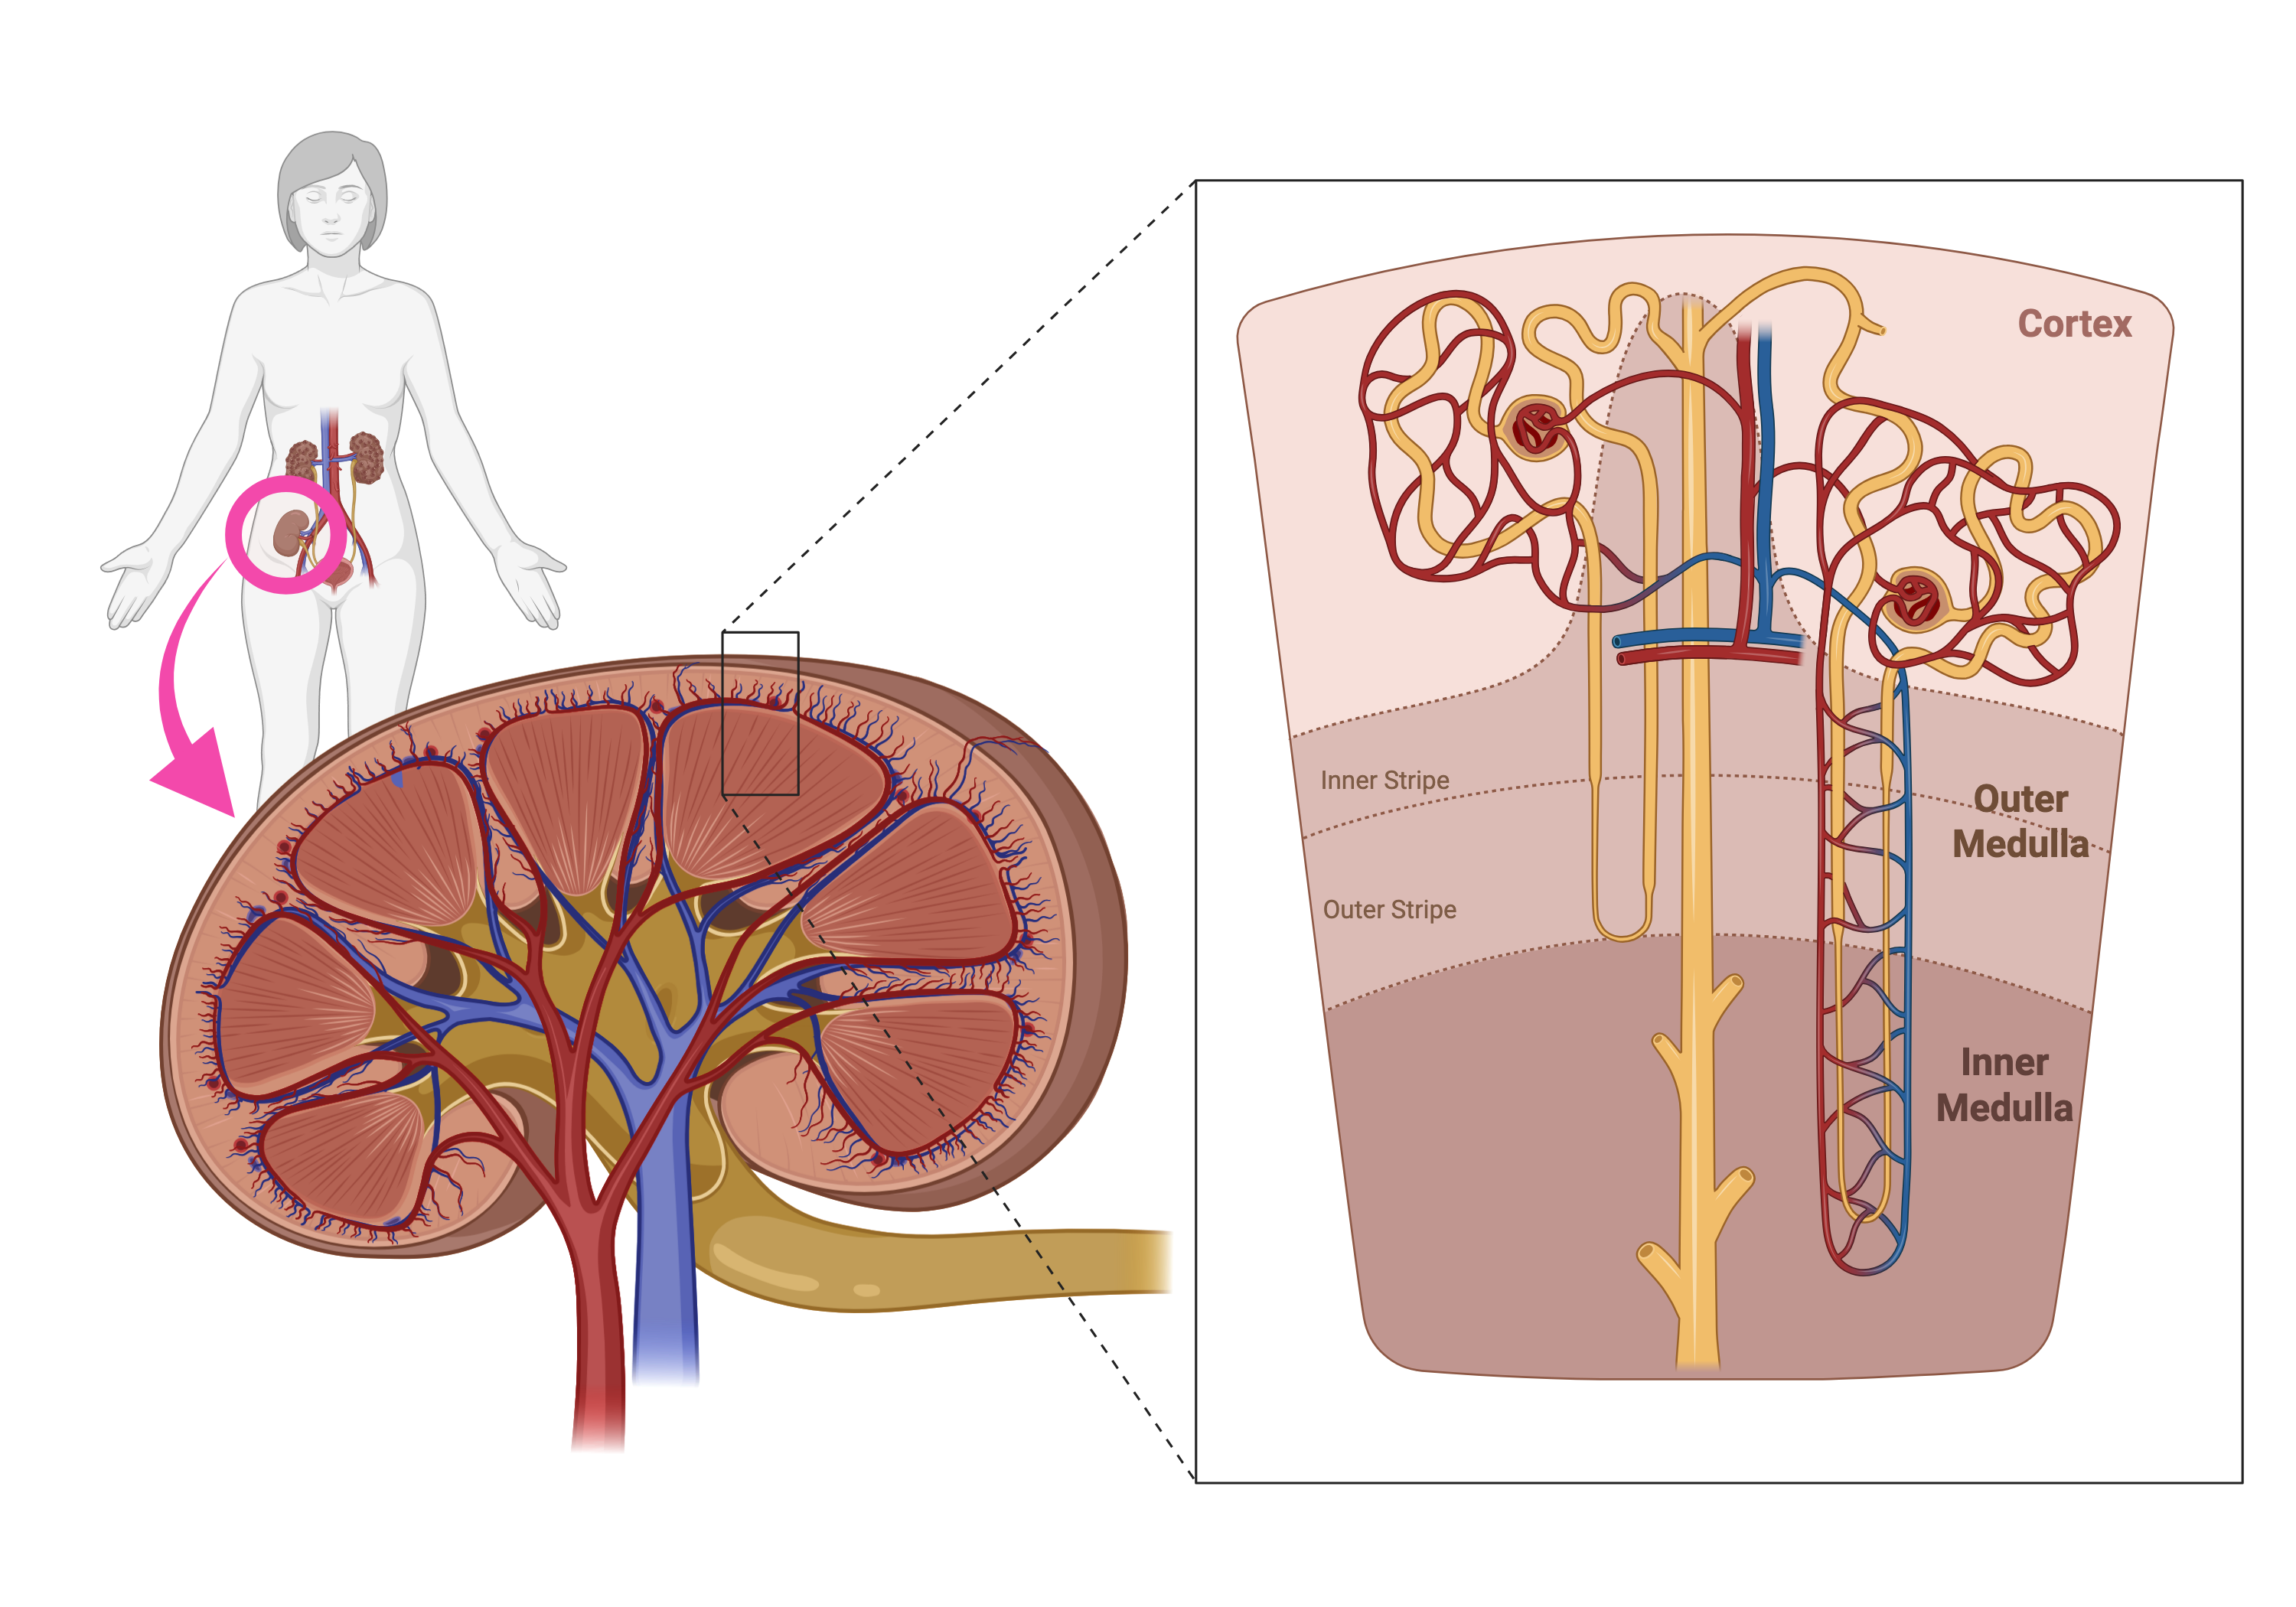
\includegraphics[width=0.85\textwidth]{parts/intro/anatomy.png}
    \caption{Macrostructural (left) and microstructural anatomy of the transplanted human kidney, with the site of a typical graft site (superficially in the anterior lower abdomen) circled in magenta. The left side shows the triangular-shaped medulla radiating out of the renal pelvis, surrounded by the cortex. The right side highlights the microstructure of the nephrons, as well as their relationship to the macroscopic features of the renal parenchyma, collecting system, and vasculature. Image created using BioRender.}
    \label{fig:anatomy}
\end{figure}

% Paragraph 2: nephrons are the functional units
%   - start in glomerulus (in cortex)
%   - proximal tubule (cortex)
%   - loop of Henle (medulla)
%   - distal tubule (cortex)
%   - collecting duct (medulla)
%   - about 1 million nephrons per kidney
%   - glomeruli perform passive filtration
%   - tubules perform active filtration, reabsorption, secretion; more metabolically demanding

Nephrons are the functional units of the kidney. Each kidney contains roughly 2 million nephrons, each of which work to filter blood and produce urine~\cite{shringi_EndStage_2026,fattah_How_2019}. A nephron begins with the glomerulus, located in the cortex, where excess solutes are passively filtered out of the bloodstream. The filtrate (i.e. partially formed urine) then passes through a series of tubules: the proximal tubule (cortex), the loop of Henle (medulla), the distal tubule (cortex), and finally the collecting duct (medulla). Throughout this process, the tubules actively reabsorb essential substances back into the bloodstream and secrete waste products into the filtrate. This active filtration process is metabolically demanding, requiring significant energy expenditure by tubular cells. While nephrons span both the cortex and medulla, kidney allograft biopsies typically focus on sampling the cortex~\cite{tsai_Current_2016} despite the medulla's functional importance and involvement in relevant pathologies~\cite{lopez_normal_2015,nankivell_Importance_2020,wei_Architecture_2015}.

% Paragraph 3: microvasculature supports nephrons
%   - glomerular capillaries
%   - afferent arteriole
%   - efferent arteriole
%   - peritubular capillaries
%   - vasa recta

The kidney's microvasculature plays a vital role in supporting nephron function. Blood enters the glomerulus through the afferent arteriole, where it is filtered by the glomerular capillaries. The filtered blood then exits via the efferent arteriole, which branches into the peritubular capillaries that surround the tubules, facilitating reabsorption and secretion processes. In the medulla, the vasa recta, a series of straight capillaries, help maintain the concentration gradient necessary for urine concentration.

% Paragraph 4: interstitial space holds it all together
%   - provides structural support
%   - mediates signaling between nephrons and vasculature
%   - ECM composition varies between cortex and medulla
%   - contains resident immune cells

Finally, the interstitial space within the renal parenchyma provides structural support to the nephrons and vasculature. It mediates signaling between these components, facilitating communication that is essential for maintaining kidney function. The extracellular matrix (ECM) composition varies between the cortex and medulla, reflecting their distinct functional roles. Additionally, the interstitial space contains resident immune cells that contribute to the kidney's defense mechanisms against pathogens and injury.

\subsection{Understanding the Banff Classification System for Renal Allograft Pathologies}

% what microstructural pathologies can exist in renal graft rejection
%   - cell morphology changes defined by Banff criteria
%     - semi-quantitative
%     - biopsy-based
%     - categorical
%     - localized to small regions of interest
%   - histological features can be grouped by location/type - explain in text, as well as a table of Banff score categories grouped by:
%     - axis 1: location
%       - interstitium
%       - vasculature (arterioles, capillaries)
%       - tubules
%       - glomeruli
%     - axis 2: injury type
%       - inflammation (total inflammation, capillaritis, tubulitis etc.)
%       - fibrosis (interstitial, glomerulosclerosis etc.)
%       - morphological changes (tubular atrophy, basal membrane thickening etc.)
%       - C4d deposition is a special case
%     - some Banff scores don't fit neatly into these categories - e.g.:
%       - interstitial fibrosis and tubular atrophy (IFTA)
%       - IFTA with interstitial inflammation (i-IFTA)
%       - IFTA with tubular injuries (t-IFTA)
%       - polyomavirus load (pvl)
%   - briefly acknowledge debates around molecular interpretation of graft dysfunction, but focus on "larger-scale" pathologies

Renal allograft biopsies are evaluated by identifying and grading various microstructural pathologies according to the Banff criteria. These criteria provide a semi-quantitative, categorical classification system for assessing changes to cellular morphology that may be associated with graft rejection and other abnormalities. The Banff system defines a diagnostic algorithm for characterizing pathologies in needle biopsy samples of the renal cortex using 17 different categories of histological features~\cite{loupy_Banff_2020}. 15 of those categories are listed in Table~\ref{tbl:banff}, grouped together by anatomical location (interstitium, vasculature, tubules, glomeruli) and injury type (inflammation, fibrosis, morphological changes). Lesion scores are defined by the extent of involvement within the sampled cortical tissue, graded on an ordinal scale from 0 to 3. Specific scores for different lesions are used alongside other contextual evidence to substantiate diagnoses that are relevant to graft dysfunction~\cite{boor_Renal_2015}.

% !TeX root = ../../main.tex

\begin{landscape}
    \singlespacing
    \begin{longtable}{
        p{1.00in} 
        p{0.30in} p{1.05in} 
        p{0.30in} p{1.20in} 
        p{0.30in} p{1.20in} 
        p{0.30in} p{1.05in}}
        \caption{Banff Classification of Renal Allograft Pathologies Grouped by Relevance to Biomechanical Alterations Except for \emph{i-IFTA} and \emph{t-IFTA}.}\\
        \label{tbl:banff}\\
        % Header
        \toprule
        \multirow{2}{=}{\textbf{Changes in/due to...}} & 
        \multicolumn{2}{l}{\textbf{Interstitia}} & 
        \multicolumn{2}{l}{\textbf{Vasculature}} & 
        \multicolumn{2}{l}{\textbf{Glomeruli}} & 
        \multicolumn{2}{l}{\textbf{Tubules}} \\
            & 
        Name & 
        Definition & 
        Name & 
        Definition & 
        Name & 
        Definition & 
        Name & 
        Definition \\
        \midrule
        \endfirsthead
        \endhead
        % Footer
        \endlastfoot
        % Row group 1: inflammation
        \multirow[t]{2}{=}{\textbf{Inflammation}} & 
        \textit{i} & 
        Interstitial \mbox{Inflammation} & 
        \textit{v} & 
        Intimal Arteritis & 
        \multirow[t]{2}{=}{\textit{g}} & 
        \multirow[t]{2}{*}{Glomerulitis} & 
        \multirow[t]{2}{=}{\textit{t}} & 
        \multirow[t]{2}{*}{Tubulitis} \\
        % Row 2: additional row 1 for inflammation
            & 
        \textit{ti} & 
        Total \mbox{Inflammation} & 
        \textit{ptc} & 
        Peritubular \mbox{Capillaritis} &
            & 
            & 
            & 
            \\
        \hline
        % Row group 2: fibrosis
        \multirow[t]{3}{=}{\textbf{Fibrosis}} & 
        \multirow[t]{3}{=}{\textit{ci}} & 
        \multirow[t]{3}{=}{Interstitial Fibrosis} & 
        \textit{cv} & 
        Vasc. Fibrous Intimal Thickening & 
        \multirow[t]{3}{=}{\textit{cg}} & 
        \multirow[t]{3}{=}{Double Contours of Glom. Basal Membrane} & 
        \multirow[t]{3}{=}{\textit{ct}} & 
        \multirow[t]{3}{=}{Tubular Atrophy} \\
        % Row 4: additional row 1 for fibrosis
            & 
            & 
            & 
        \textit{ah} & 
        Arteriolar \mbox{Hyalinosis*} & 
            & 
            & 
            & 
            \\
        % Row 5: additional row 2 for fibrosis
            & 
            & 
            & 
        \textit{aah} & 
        Hyaline Arteriolar Thickening* & 
            & 
            & 
            & 
            \\
        \hline
        % Row group 3: other
        \textbf{Other} & 
            & 
            & 
        \textit{C4d} & 
        C4d Staining on PTC Endothelia or Medullary Vasa Recta & 
        \textit{mm} & 
        Mesangial \mbox{Matrix} Expansion* & 
        \textit{pvl} & 
        Polyomavirus Nephropathy \\
        \bottomrule
    \end{longtable}
    \par\vspace{0.5em}
    \noindent*: Lesion types with asterisks denote purely descriptive changes that are not used for classifying rejection types in the Banff system.
\end{landscape}


The Banff system includes six numbered categories of diagnoses for renal allograft pathologies. The categories include those that are focused on AMR (a majority of Category 2), TCMR (Category 4), and borderline TCMR (Category 3), as well as those that are not directly related to rejection (Categories 1 for normal findings or nonspecific changes, and Category 6 for non-rejection-related findings such as polyomavirus nephropathy). However, Category 5 is of special relevance to this work: interstitial fibrosis and tubular atrophy (IFTA). IFTA is a common finding in chronic graft dysfunction and is characterized by the presence of fibrosis in the interstitial space along with atrophy of the renal tubules. In fact, the two Banff lesion scores not mentioned in Table~\ref{tbl:banff}, inflammation in the presence of IFTA (\emph{i-IFTA}) and tubulitis in the presence of IFTA (\emph{t-IFTA}), uniquely depend on the presence of IFTA for their definition. These six diagnostic categories, with exception of Category 1 with non-IFTA findings, are not mutually exclusive; a single biopsy can receive multiple diagnoses if the relevant criteria are met. Therefore, findings like IFTA can be found on their own, but they can also co-occur with - and may even act as risk factors of poorer graft survival rates for - other diagnoses such as AMR or TCMR.

As the complex procedure for identifying and classifying these microstructural pathologies suggests, renal allograft dysfunction and rejection are multifaceted processes that can manifest through a variety of histological changes. Recent works have sought to better understand these processes by integrating molecular information with traditional histological assessments~\cite{bloom_CellFree_2017,sugi_Imaging_2019,goutaudier_Evaluation_2024}. While these molecular approaches can provide valuable insights into the underlying mechanisms of graft dysfunction, this dissertation aims to be more practically focused. Therefore, the discussion will primarily center around the larger-scale pathologies defined by the Banff criteria, particularly those related to inflammation and fibrosis, which are more directly relevant to clinical diagnostics and patient management.

\subsection{A Multi-Scale Perspective of Kidney Pathologies}

% - Paragraph 1: view renal parenchyma microstructure through biomechanics lens
%   - consider renal parenchyma as composite material made of multiple components
%   - nephrons (tubules + glomeruli) = functional core that essentially acts as load-bearing structures
%   - microvasculature (arterioles + capillaries) = cross-link network with roles in perfusion and nutrient delivery
%   - interstitial space (ECM + fibroblasts + immune cells) = matrix that supports other two components
%   - biological tissue is generally considered to be viscoelastic
%     - EXAMPLE: kidney tissue viscoelasticity from literature

To connect the microstructural pathologies defined by the Banff criteria to biomechanical properties that can be noninvasively assessed using ultrasound-based techniques, it is helpful to understand the renal parenchyma through a biomaterials lens. Considering that the renal parenchyma is primarily composed of orientationally organized nephrons, a dense microvasculature network, and a supportive interstitial matrix, one can reasonably interpret it as a fiber-reinforced composite material~\cite{karimi_Measurement_2017,gennisson_Supersonic_2012}. Specifically, the tubules of nephrons can be viewed as load-bearing structures that provide mechanical integrity to the tissue, while the microvasculature (glomeruli, peritubular capillaries etc.) acts as a cross-link network that distributes mechanical loads and facilitates nutrient delivery. The interstitial space, which houses the extracellular matrix, resident immune cells, and lymphatic features, serves as the matrix phase that binds the other two components together and maintains overall tissue structure. Biological tissues, including the renal parenchyma, are generally considered to exhibit viscoelastic behavior, meaning they display both elastic (solid-like) and viscous (fluid-like) responses to mechanical loading. Prior studies have characterized the viscoelastic properties of kidney tissue~\cite{karimi_Measurement_2017,liu_Effect_2017,pirsoltan_Investigation_2025,vasconcelos_Kidney_2024}, demonstrating that these properties can be influenced by various factors such as hydration status, temperature, and pathological changes. 

% - Paragraph 2: histological changes and viscoelastic changes can be related
%   - in that model...
%     - tubular injury = changes to structural integrity of nephrons
%     - vascular injury = changes to fiber-matrix relationship
%     - interstitial changes = changes to matrix material properties
%   - nephrons are oriented radially from cortex to medulla
%   - therefore, renal parenchyma can be considered transversely isotropic
%   - thus, histological changes may lead to changes in viscoelastic anisotropy
%   - problem can be inverted; detecting viscoelastic changes may provide insight into underlying histological changes

Within this framework, the various histological changes defined by the Banff criteria can be interpreted as alterations to the biomechanical properties of the renal parenchyma. For instance, tubular injuries such as tubular atrophy can be viewed as disruptions to the structural integrity of the nephrons, potentially leading to decreased stiffness and altered viscoelastic responses. Likewise, vascular injuries such as capillaritis and arteritis, may affect the fiber-matrix relationship within the tissue, influencing how mechanical loads are distributed and absorbed. Interstitial changes, such as interstitial inflammation and fibrosis, can modify the material properties of the matrix phase. Given that nephrons are oriented radially from the cortex to the medulla, the renal parenchyma can be considered to be transversely isotropic (TI) in three dimensions - that is, its mechanical properties differ along one axis (along nephrons) while it is isotropic in the two orthogonal axes (perpendicular to nephrons). Furthermore, as mentioned in Section~\ref{sec:anatomy}, the composition of the renal parenchyma varies between the cortex and medulla, suggesting that disease processes may also exhibit viscoelastic heterogeneity across anatomical regions. Consequently, histological changes that affect the microstructure of the renal parenchyma may lead to detectable alterations in its viscoelastic anisotropy and heterogeneity. This relationship, then, may be inverted: by noninvasively assessing changes in the viscoelastic anisotropy and heterogeneity of the parenchyma of renal allografts, it may be possible to infer underlying histological changes associated with graft dysfunction and rejection - be it AMR, TCMR, IFTA, or other pathologies defined by the Banff criteria.

\subsection{Implications for Ideal Diagnostic Approaches}

% - Paragraph 1: ideal diagnostic approach should noninvasively assess information about microstructure of renal parenchyma
%   - noninvasive imaging preferred over biopsy because:
%     - avoids risks associated with invasive procedures
%     - allows for more frequent longitudinal monitoring
%     - captures spatial heterogeneity of graft pathology
%     - reduces sampling error inherent in biopsies
%   - ideal imaging modality should provide information about:
%     - inflammation vs. fibrosis
%     - severity of microstructural changes
%     - spatial distribution of pathologies
%     - temporal progression of graft dysfunction
%   - biomechanical properties (e.g. viscoelasticity) may serve as useful biomarkers because they reflect underlying microstructural changes

It is crucial to recognize that the Banff criteria focuses on microstructural changes that are localized to small regions of interest within the renal cortex. As an organ that is heterogeneous both in terms of macrostructure and cellular phenotypes, the kidney can exhibit significant spatial variability in pathology. This heterogeneity poses challenges for biopsy-based assessments, as the sampled tissue may not fully represent the overall state of the graft. As such, an ideal adjunct to needle biopsies for monitoring renal allografts would be a noninvasive imaging modality capable of providing information about the microstructure of the renal parenchyma. Noninvasive imaging techniques offer several advantages over biopsies, including the ability to avoid risks associated with invasive procedures, facilitate more frequent longitudinal monitoring, capture spatial heterogeneity of graft pathology, and reduce sampling error inherent in biopsies. An ideal imaging modality should provide insights into key aspects of graft health such as the the presence of inflammation and fibrosis, the severity of microstructural changes, the spatial distribution of pathologies, and the temporal progression of graft dysfunction. Given that biomechanical properties like viscoelasticity are influenced by underlying microstructural changes, they may serve as useful biomarkers for noninvasively assessing graft health.

% - Paragraph 2: viscoelastic properties can provide biologically relevant information about tissue microstructure
%   - inflammation = cellular infiltration, edema, increased vascular permeability
%     - likely leads to decreased stiffness, increased viscosity
%   - fibrosis = excess ECM deposition, scar tissue formation
%     - likely leads to increased stiffness, decreased viscosity
%   - Banff criteria distinguishes AMR, TCMR etc. based on presence of inflammation, fibrosis, other lesions
%   - thus, identification of inflammation and/or fibrosis via mechanical properties may act as biomarkers for graft pathologies including rejection

Viscoelasticity measurements can provide biologically relevant information about tissue microstructure that may be indicative of specific pathological processes. For example, inflammation is characterized by cellular infiltration, edema, and increased vascular permeability, which can lead to decreased tissue stiffness and increased viscosity~\cite{kimondo_Mechanical_2024}. Conversely, fibrosis involves excess extracellular matrix deposition and scar tissue formation, typically resulting in increased stiffness~\cite{wenger_Mechanical_2007}. Furthermore, the Banff \emph{i-IFTA} score, or the combined presence of interstitial inflammation where IFTA is present, is a particularly pertinent indicator of graft dysfunction and survival~\cite{gago_Kidney_2012,nankivell_causes_2018}. Since the Banff criteria considers information about inflammation and/or fibrosis to distinguish between different types of graft pathologies such as AMR and TCMR, the ability to identify these conditions through changes in mechanical properties may serve as valuable biomarkers for diagnosing and monitoring kidney allograft health.

% - conclusion: an ideal approach to gaining insight into underlying microstructural changes associated with graft dysfunction and rejection involves noninvasive assessments of viscoelastic properties of renal parenchyma

In conclusion, an ideal approach to gaining insight into the underlying microstructural changes associated with graft dysfunction and rejection involves noninvasive assessments of the viscoelastic properties of the renal parenchyma such that inflammation and/or fibrosis may be distinguished. By leveraging the relationship between biomechanical properties and histological changes, such imaging techniques have the potential to enhance our ability to monitor graft health and improve patient outcomes.


% !TeX root = ../../main.tex

\section{Acoustic Radiation Force-Based Elastography}

\subsection{Relevant Ultrasound Physics}

% Paragraph 1: tissue scatterers encode tissue/material motion
%   - Ultrasound imaging relies on backscattered signals from tissue microstructure
%   - Scatterers are small (subresolution) inhomogeneities in acoustic impedance
%   - Scatterers are spatially randomly distributed but stationary
%   - Therefore, temporal changes in scatterer positions reflect tissue motion

Ultrasound elastography techniques leverage the ability of ultrasound imaging to detect tissue motion and infer mechanical properties from that motion~\cite{nenadic_Ultrasound_2019}. This is fundamentally possible because biomedical ultrasound imaging relies on tissue to reflect acoustic pulses beyond the range of human hearing (typically at a frequency on the order of 1--20 MHz). Ultrasound imaging involves the use of transducers, or materials that convert electrical energy into acoustic (mechanical) energy and vice versa, to both generate and receive these acoustic pulses. Transmitted acoustic pulses propagate through soft tissue, where the speed of sound is known to be on the order of 1540 m/s, and are partially reflected back to the transducer by small (subresolution) inhomogeneities in material properties~\cite{trahey_Properties_1988}. These inhomogeneities, known as scatterers, arise from spatial variations in acoustic impedance (the product of material density and speed of sound) due to differences in tissue composition and structure. Scatterers are spatially distributed in a random manner but stationary over time~\cite{trahey_Properties_1988}. Therefore, temporal changes in scatterer positions reflect motion that takes place in tissue. By analyzing the backscattered signals over time, ultrasound imaging can track tissue motion with high spatial and temporal resolution~\cite{kasai_RealTime_1985,loupas_Experimental_1995,ashikuzzaman_Displacement_2024}.

% Paragraph 2: motion encodes material properties
%   - Tissue motion can be induced extrinsic (surface level or at depth) or intrinsic (i.e. physiological motion)
%   - Relationship between applied force (stress) and resulting motion (strain) reflects material properties
%   - Stress-strain relationship most easily encoded as linearly elastic material property: Young's modulus
%   - Change in apparent Young's modulus over time reflects viscoelastic properties
%     - multiple models exist to describe viscoelasticity (e.g. Kelvin-Voigt, Maxwell)
%   - Ultrasound elastography leverages this relationship to infer tissue mechanical properties from measured motion

Tissue motion can be induced either extrinsically, through external forces applied at the surface or at depth within the tissue, or intrinsically, through physiological motion such as cardiac pulsation or respiratory movement. The relationship between the applied force (stress) and the resulting motion (strain) reflects the material properties of the tissue. In the simplest case, this can be considered a linear relationship where the proportionality constant is the stiffness - i.e. Young's modulus. The Young's modulus describes how much a material deforms in response to an applied force, with stiffer materials exhibiting less deformation. However, biological tissues often exhibit viscoelastic behavior, meaning that their mechanical response to an applied force depends not only on the magnitude of the stress but also on the duration over which it is applied. This time-dependent behavior can be characterized by changes in the apparent Young's modulus over time, providing insights into the viscoelastic properties of the tissue. Various models exist to describe viscoelasticity, including the Kelvin-Voigt and Maxwell models, which account for both elastic and viscous components of tissue behavior. Ultrasound elastography techniques leverage this relationship between stress and strain to infer tissue mechanical properties from measured motion, enabling noninvasive assessments of tissue stiffness and viscoelasticity.

% Paragraphs 3: anatomy of an ultrasound elastography workflow
%   - Step 1: apply force to tissue
%     - Examples:
%       - External compression (manual or mechanical)
%       - Acoustic Radiation Force (ARF) push
%       - Vibratory sources (e.g. shaker)
%       - Passive (i.e. physiological motion)
%       - Others (magnetic, optical etc.)
%     - ARF is useful for deep, localized, controlled force application
%     - ARF due to acoustic nonlinearity, momentum transfer from compressive wave
%   - Step 2: track resulting tissue motion using ultrasound imaging
%     - Multiple pulse emissions create an ensemble
%     - Backscatter phase shifts reflect scatterer displacements
%     - Motion tracking algorithms (Kasai, Loupas, NCC etc.) estimate displacements
%     - Displacements are never perfect
%       - Decorrelation = loss of correlation between echoes due to out-of-plane motion, deformation, noise
%       - Cramer-Rao lower bound describes minimum variance of unbiased estimators
%       - Deformation (displacement) gradient leads to underestimation of displacements
%       - Experimental demonstration: Czernuszewicz et al.
%   - Step 3: analyze motion data to estimate mechanical properties
%     - can involve strain, particle velocity, etc.
%     - may or may not involve beamforming + envelope-detection
%     - multiple analysis techniques exist - including where to track
%     - quickly transition into next subsection

Ultrasound elastography workflows primarily involve three key steps. The first step is to apply a force to the tissue of interest. This can be achieved through various means, including external compression (either manual or mechanical)~\cite{garra_Elastography_2015,ophir_Elastography_1991}, Acoustic Radiation Force (ARF) pushes~\cite{garra_Elastography_2015,sarvazyan_Shear_1998,nightingale_feasibility_2001}, vibratory sources~\cite{lerner_SonoElasticity_1988,parker_Tissue_1990,sandrin_Transient_2003}, or passive methods that leverage physiological motion~\cite{gallot_Passive_2011,catheline_Tomography_2013,vappou_Pulse_2010}. ARF is particularly useful for deep, localized, and controlled force application, as it generates a focused acoustic pulse that induces localized tissue displacement through acoustic nonlinearity and momentum transfer from the compressive wave.

The second step involves tracking the resulting tissue motion using ultrasound imaging. This is typically accomplished by emitting multiple ultrasound pulses to create an ensemble of backscattered signals. The phase shifts in these backscattered echoes reflect the displacements of scatterers within the tissue. Various motion tracking algorithms, such as Kasai~\cite{kasai_RealTime_1985}, Loupas~\cite{loupas_Experimental_1995}, and normalized cross-correlation (NCC)~\cite{pinton_Rapid_2006}, are employed to estimate these displacements. However, it is important to note that displacement estimates are never perfect. The most important factors that affect the accuracy of displacement estimates include decorrelation, which refers to the loss of correlation between echoes caused by out-of-plane motion, deformation, and noise. However, other factors such as the bandwidth and signal-to-noise ratio (SNR) of the ultrasound system also play a role~\cite{walker_fundamental_1995}. The Cramer-Rao lower bound describes the minimum variance of unbiased estimators, providing a theoretical limit on the accuracy of displacement estimates~\cite{mcaleavey_Estimates_2003,dhanaliwala_Assessing_2012}.

Crucially, the idea of a "perfect" displacement estimate is only possible where there is a single point in space moving rigidly. In reality, tissue deforms over a continuous volume; tissue always deforms across a displacement gradient. Since ultrasonic tracking pulses (as with any other imaging modality) have a finite spatial resolution, the displacement estimate within a resolution cell volume (i.e. its point spread function, or PSF) is effectively an average of displacements across that cell~\cite{walker_fundamental_1995,mcaleavey_Estimates_2003,palmeri_Ultrasonic_2006}. Czernuszewicz \emph{et al.} experimentally demonstrated this phenomenon in a simple situation: when an ARF push is applied onto an acoustically scattering but optically transparent phantom with a glass bead at the focal point of the push, acoustic displacement estimates underestimated the true displacement of the bead due to the presence of a displacement gradient in the surrounding material~\cite{czernuszewicz_Experimental_2013}. This displacement gradient effect, crucially, is also materially dependent; since stiffer materials deform less and recover faster from the same applied force compared to softer materials, displacement estimation errors due to displacement gradients also encode information about underlying material properties.

The final step of ultrasound elastography involves analyzing the motion data to estimate mechanical properties of the tissue. This analysis can involve various metrics such as strain rate, particle velocity, shear wave group and phase speeds, or even features inferred through machine learning approaches~\cite{gennisson_Rheology_2014,wiseman_parametric_2020,jin_SweiNet_2022,chen_ShearWave_2023} - each of which may be further modified with various beamforming approaches~\cite{song_CombPush_2013,ahmed_PlaneWave_2018}. Multiple analysis techniques exist, each with its own approach to processing the motion data and determining where to track displacements within the tissue. The choice of analysis technique can significantly impact the accuracy and reliability of the estimated mechanical properties, leading to a diverse array of ultrasound elastography methods that have been developed to suit different clinical applications and research needs.

\subsection{On-Axis ARF-based Elastography}

% Paragraph 1: introduce ARFI imaging
%   - ARFI = Acoustic Radiation Force Impulse imaging
%   - Uses short-duration ARF push to induce localized displacement
%   - Tracks on-axis displacements at push location
%   - Initial development by Nightingale et al. in early 2000s
%   - Used clinically in liver fibrosis staging (e.g. Siemens Virtual Touch)

ARF-based techniques of ultrasound elastography can be broadly categorized into on-axis and off-axis methods, depending on where tissue motion is tracked relative to the location of the ARF push. On-axis techniques focus on tracking displacements directly at the push location. The primary approach in this category is Acoustic Radiation Force Impulse (ARFI) imaging. ARFI imaging employs a short-duration ARF push to induce localized tissue displacement at a specific location, and then tracks the resulting on-axis displacements at that push location. This technique was initially developed by Nightingale \emph{et al.} in the early 2000s~\cite{nightingale_feasibility_2001,nightingale_Acoustic_2002}, and has since been adopted in clinical applications such as liver fibrosis staging~\cite{nierhoff_efficiency_2013,shiina_WFUMB_2015}, thyroid cancer classification~\cite{zhan_Acoustic_2015,zhang_Acoustic_2015}, and breast lesion characterization~\cite{balleyguier_Breast_2013}. Commercial implementations of ARFI imaging, such as Siemens' Virtual Touch technology, have made this technique widely accessible in clinical settings.

% Paragraph 2: limitations of ARFI-based metrics
%   - ARF push amplitude unknown
%   - Peak displacement works qualitatively
%   - Other metrics too SNR-sensitive (e.g. time to recovery), temporally constricting (time-to-peak) etc.
%   - Viscosity confounds all metrics

However, ARFI faces several limitations as a method for estimating tissue mechanical properties. One of the primary challenges is that the amplitude of the ARF push is typically unknown, precluding its use for quantitative elasticity estimation. As a result, ARFI-derived metrics, such as peak displacement, are often used qualitatively to differentiate between softer and stiffer tissues. While other ARFI-derived metrics such as the time to peak displacement or time to recovery have been proposed~\cite{sarvazyan_Shear_1998,nightingale_Acoustic_2011}, they are often highly sensitive to signal-to-noise ratio (SNR) or may occur over a time scale that is too short to be reliably measured, limiting their clinical utility. Additionally, the presence of tissue viscosity further complicates the interpretation of ARFI metrics, as viscous effects can alter the displacement response in ways that are not directly related to tissue stiffness. These limitations highlight the need for alternative approaches that can provide more robust and quantitative assessments of tissue mechanical properties.

\subsection{Off-Axis Shear Wave-based Elastography}
\label{sec:about_offaxis}

% Paragraph 1: introduce shear wave elastography
%   - Shear waves = transverse waves induced by ARF push
%   - Shear wave speed related to shear modulus (and thus Young's modulus)
%   - Multiple techniques exist:
%     - SWEI (Shear Wave Elasticity Imaging)
%     - SDUV (Shearwave Dispersion Ultrasound Vibrometry)
%     - SSI (Supersonic Shear Imaging)
%     - Others
%   - Also used in wide variety of clinical applications
%   - Shear wave speed can be used to infer tissue viscosity

Shear wave-based techniques represent another major category of ARF-based ultrasound elastography methods, characterized by their focus on tracking tissue motion off-axis from the ARF push location. Shear waves are transverse waves that propagate laterally through tissue following an ARF push. Similar to the relationship between compressional wave speed and bulk modulus, shear wave speeds are governed by the shear modulus of the material. Therefore, measurements of shear wave speed can be used to infer tissue stiffness, typically represented by Young's modulus in isotropic and linearly elastic materials~\cite{sarvazyan_Shear_1998}. Several shear wave elastography techniques have been developed including Multi-Track-Location Shear Wave Elasticity Imaging (MTL-SWEI)~\cite{sarvazyan_Shear_1998,nightingale_Shearwave_2003}, Single-Track-Location Shear Wave Elasticity Imaging (STL-SWEI)~\cite{elegbe_Single_2013,hollender_Single_2015}, and Supersonic Shear Imaging (SSI)~\cite{bercoff_Supersonic_2004}. These methods have been widely applied in various clinical contexts, such as liver fibrosis assessment~\cite{frulio_Evaluation_2013,nenadic_Ultrasound_2019}, breast lesion characterization~\cite{balleyguier_Breast_2013}, and musculoskeletal evaluations~\cite{ryu_Current_2017}.

Shear wave speed measurements can also provide insights into tissue viscosity. Techniques such as Shearwave Dispersion Ultrasonic Vibrometry (SDUV)~\cite{chen_Shearwave_2009} or group shear wave speed measurement~\cite{kim_Prediction_2024,rouze_Characterization_2018,yuan_Ultrasound_2024} to analyze shear wave dispersion, or the frequency-dependent variation in shear wave speed, to estimate viscoelastic properties. This analysis enables the characterization of both elastic and viscous components of tissue behavior using the same data acquisition pipeline, offering a more comprehensive understanding of tissue mechanics.

% Paragraph 2: limitations of shear wave-based metrics
%   - Must detect shear waves off-axis; spatial averaging is inherent
%   - Shear wave speed confounded by:
%     - Heterogeneity
%     - Anisotropy
%     - Geometric complexity (wave guiding, reflections, dispersion etc.)
%   - Particularly problematic in kidneys due to:
%     - Heterogeneity (in multiple scales)
%     - Anisotropy (when acquisition poorly controlled in beam sequencing and in acquisition protocol)

However, shear wave-based techniques also face significant challenges that can confound their ability to accurately estimate tissue mechanical properties. Since shear waves must be detected by measuring displacements across multiple tracking positions relative to the push location, the material property estimates derived from shear wave speed inherently involve an assumption that the tissue is homogeneous over the sampling region. This spatial averaging can lead to inaccuracies in heterogeneous tissues, as well as in situations where elastic anisotropy, imaging artifacts such as clutter or reverberation, and geometric complexity such as wave guiding effects, reflections, and dispersion may take place. These confounding factors are particularly problematic in organs like the kidney, which exhibit significant heterogeneity at multiple scales (e.g., cortex vs. medulla) and anisotropy. Shear wave speed measurements have also been shown to be sensitive to imaging parameters, ARF push amplitudes, and acquisition protocols, further complicating their clinical application~\cite{palmeri_Radiological_2021,elmeliegy_Correlationbased_2023}.

Shear wave-based techniques in the kidney have also been demonstrated to be an imperfect tool for assessing renal pathology, highlighting the variability and inconsistency in reported shear wave speed or elastic (shear or Young's moduli) values across different studies. Notably, many studies have reported conflicting methods for reporting results. This includes inconsistencies between reporting shear wave speeds versus derived elastic moduli (which assumes linear, isotropic elasticity)~\cite{ce_Ultrasound_2023,ng_Shear_2024,urban_Novel_2021}, how patients are positioned during imaging~\cite{ce_Ultrasound_2023}, what system is used to perform imaging~\cite{ng_Shear_2024}, whether measurements are made using image-based regions of interest (ROI) or pointwise samples~\cite{sandhya_Role_2025}, how image quality and artifact rejection are handled~\cite{ce_Ultrasound_2023,barr_Can_2020}, and what biomarkers are used for comparison~\cite{alnazer_Recent_2021,cao_Shear_2023}. Renal perfusion is also known to affect shear wave speed measurements, though the directionality of this effect and the proper approach to comparing perfusion metrics remains unclear~\cite{alnazer_Recent_2021,filipov_Investigating_2024,leong_Comparison_2019,lim_Shear_2021,ozkan_Interobserver_2013,urban_Novel_2021}. These inconsistencies complicate the interpretation and comparison of results across studies, hindering the establishment of standardized protocols and reference values for renal shear wave elastography.

Furthermore, the approach of measuring shear wave speeds in the kidney has been inconsistent in the literature to the point that their utility as a biomarker is questionable. Significant variations exist in where previous works placed ROIs in terms of kidney orientation (along vs. across the long axis of the kidney), gross anatomical position (superior pole, inferior pole, or median), and depth (whether multiple measurements are taken at matching depths) have varied widely~\cite{barr_Can_2020,ce_Ultrasound_2023,ng_Shear_2024,urban_Novel_2021}. Additionally, there is no consensus on how to define the ROI within the kidney structure itself; some works focus on the cortex alone, while others distinguish between the inner and outer cortex, and still others lump together the cortex and medulla into a universal label of renal parenchyma~\cite{ce_Ultrasound_2023}. Because of the aforementioned need for shear waves to develop and propagate over a scale of millimeters to centimeters, it is reasonable to expect that shear wave speed measurements would differ based on anatomical location (e.g. inconsistent averaging across the corticomedullary junction) and orientation (e.g. erroneous averaging of shear wave speeds taken along different material orientations). Therefore, the inability to standardize anatomical locations and orientations is particularly problematic for shear wave-based techniques in the kidney.~\footnote{
    Magnetic resonance imaging (MRI)-based elastography (MRE) has also been applied to assess renal allograft pathologies~\cite{lee_MR_2012,kirpalani_Magnetic_2017} but also suffers from reproducibility issues. This may be due to the use of the entire renal cortex (or even the whole parenchyma) for ROIs (e.g. example ROIs in \cite{kennedy_Magnetic_2020}, \cite{chauveau_Magnetic_2022}, and \cite{shatil_Magnetic_2022}). Since this challenge regarding heterogeneity and anisotropy is shared with ultrasound shear wave elastography, MRE is not detailed further in this dissertation.
}

Together, these limitations suggest that while shear wave-based elastography techniques have shown promise in assessing tissue mechanical properties, their application in the kidney is fraught with challenges that must be carefully considered. The inherent assumptions of homogeneity and isotropy, coupled with the complex anatomy and physiology of the kidney, necessitate the development of alternative approaches that can provide more reliable and robust assessments of renal tissue mechanics - especially one where the influence of heterogeneity and anisotropy can be explicitly accounted for.

\subsection{Viscoelastic Response (VisR) Elastography}

% Paragraph 1: introduce VisR elastography
% - VisR = Viscoelastic Response elastography
% - Uses dual ARF pushes to induce displacements
% - Tracks on-axis displacements at push location
% - Analyzes displacement profile over time to estimate viscoelastic parameters
% - Like ARFI, on-axis
% - Like shear wave, parameterizes viscoelastic properties (through MSD model)
%   - maybe also allude to state space, QVisR, other approaches from Joey and Lucas?
% - VisR metrics qualitative as biomarkers (they characterize displacement profiles, but do not necessarily quantify information about underlying tissue)

In response to the limitations of both ARFI and shear wave-based techniques, Viscoelastic Response (VisR) elastography~\cite{selzo_Viscoelastic_2013} was developed as an on-axis ARF-based method that aims to provide semi-quantitative assessments of tissue viscoelastic properties. VisR elastography employs two ARF excitations in short succession to induce localized tissue displacements at the push location, similar to ARFI imaging. However, instead of relying solely on the peak displacement, VisR characterizes viscoelastic properties of the underlying material by parameterizing the entire displacement profile over time. By fitting the measured displacement data to a mechanical model such as the one-dimensional mass-spring-damper (MSD) model~\cite{selzo_Quantitative_2016}, VisR can extract parameters related to both elasticity and viscosity of the tissue~\cite{hossain_Viscoelastic_2020}.

% Paragraph 2: VisR as a biomarker
% - Define VisR relative elasticity (RE) / relative viscosity (RV)
%   - RE/RV are related to true material properties divided by unknown ARF push magnitude
%   - thus, RE/RV are semi-quantitative biomarkers
% - If A can be assumed constant, ratios of RE/RV can be treated as quantitative
%   - RR = regional ratio (heterogeneity)
%   - DoA = degree of anisotropy (anisotropy)

VisR fit parameters can be used to derive semi-quantitative biomarkers that have been found to correlate with tissue mechanical properties. Two key metrics derived from VisR are the relative elasticity (RE) and relative viscosity (RV), which represent the underlying shear elastic and viscous moduli normalized by the unknown ARF push magnitude. Since the ARF push magnitude is not directly measured, RE and RV cannot be treated as absolute quantitative measures of tissue properties, leading the metrics to be \emph{semi}-quantitative in nature.

However, if the ARF push magnitude can be assumed to be constant across different measurements, ratios of RE and RV can be treated as quantitative indicators of tissue heterogeneity and anisotropy. For instance, the regional ratio (RR) can be used to assess heterogeneity by comparing RE or RV values across different regions of interest. Since the ARF push magnitude is canceled out in the ratio, RR provides a quantitative measure of relative stiffness or viscosity between spatial regions. Likewise, the degree of anisotropy (DoA) can be calculated by comparing RE or RV values obtained from different imaging orientations to determine the extent of directional dependence in tissue mechanical properties.\footnote{
    Note that RR and DoA are not metrics that are exclusive to VisR elastography. Similar ratio-based metrics can also be derived from other techniques such as shear wave speed measurements from MTL-SWEI or SDUV, as well as other on-axis techniques such as ARFI peak displacement. However, VisR's on-axis tracking and viscoelastic parameterization provide a unique approach to obtaining these metrics.
} 

% Paragraph 3: prior work on VisR elastography
% - Initial development by Mallory, Chris, Murad, and Gabriela/Anna
% - Multiple ex vivo and in vivo studies
%   - muscle (GRMD in dogs, DMD in children)
%   - breast cancer
%   - kidney
% - Previous renal studies were:
%   - In vivo, exteriorized
%   - In vivo, humans - but for small sample size
%     - differentiated various renal pathologies but small sample size

VisR elastography was initially developed by Selzo and Gallippi~\cite{selzo_Viscoelastic_2013} using a Voigt material model to characterize viscoelastic response. Subsequent studies have expanded upon this work, applying VisR elastography in various ex vivo and in vivo contexts. Notably, VisR has been utilized to assess muscle pathology in both Golden Retriever Muscular Dystrophy (GRMD) in dogs~\cite{moore_Computational_2018} and Duchenne Muscular Dystrophy (DMD) in children~\cite{moore_Vivo_2018}, demonstrating its potential for evaluating muscular disorders. Additionally, VisR has been demonstrated to differentiate between benign and malignant breast lesions \emph{in vivo} in humans, highlighting its utility in oncological applications~\cite{phillips_VisR_2025}. Furthermore, VisR has been shown to be robust to changes in renal perfusion in an \emph{in vivo} porcine model of renal ischemic reperfusion injury~\cite{hossain_Viscoelastic_2018}, a finding that was also noted in humans using SWEI~\cite{gao_Ultrasound_2020} and in a preclinical implementation of SDUV~\cite{amador_Shearwave_2011}.

% - Paragraph 4: what's not done yet
%   - longitudinal study
%   - histological correlation over larger sample size
%   - explicit comparison to Banff scores
%   - investigating VisR-like approaches that relax assumptions about displacement profile parameterization (our first hint at DoPIo)

Previous works have also explored the application of VisR in kidneys, with studies conducted in exteriorized porcine kidneys \emph{in vivo}~\cite{hossain_Viscoelastic_2018} as well as in a small cohort of human renal transplant patients~\cite{hossain_Evaluating_2018}. In the former study, VisR, MTL-SWEI, and SDUV imaging were performed in a porcine model of ischemic reperfusion injury. This study demonstrated that DoA were significantly different between injured and contralateral kidneys using VisR RE metrics in the cortex and medulla, as well as in the medulla using VisR RV-based DoA. This was comparable to how DoA derived from shear elasticity estimates using SDUV were also significantly different between injured and contralateral kidneys in both cortex and medulla, as well as MTL-SWEI shear wave speed-based DoA in the medulla. This result also corresponds to DoA changes made using ARFI peak displacements both in the cortex and medulla, which has also been shown to reflect elastic anisotropy in TI materials~\cite{hossain_Acoustic_2017,hossain_Quantitative_2022}.

For the study on human renal transplant patients conducted by Hossain \emph{et al.}~\cite{hossain_Evaluating_2018}, VisR elastography was performed \emph{in vivo} on a small cohort of 19 patients who underwent clinically indicated biopsies as well as 25 volunteers who received renal allografts but did not undergo any biopsies. The biopsies were found to have various renal pathologies including acute rejection (nonspecific between AMR and TCMR), chronic allograft nephropathy, BK virus nephropathy, and glomerulonephritis. In this study, RE-based RR between the pelvis and parenchyma were found to be significantly different between non-biopsied controls and patients with moderate vascular disease, as well as with patients with mild interstitial scarring. RV-based RR between the pelvis and parenchyma were also significantly different between non-biopsied controls and patients with moderate vascular disease. This suggests that metrics derived from VisR RE and RV parameters may serve as potential biomarkers for distinguishing pathologies in the renal parenchyma that are relevant to graft dysfunction. It should be noted, however, that DoA using RE or RR were not reported in this work, and the patient sample sizes were relatively small. Furthermore, this study did not consider longitudinal monitoring of renal allografts over time or differentiate the renal cortex from the medulla in the parenchyma. In terms of clinical correlations, biopsy results were only categorized based on the clinical diagnosis rather than Banff scores. As such, while this study provided initial evidence regarding VisR's potential biological relevance in assessing renal allograft health, the utility of VisR for longitudinally monitoring renal allograft health is yet to be investigated.

\subsection{Challenges of Existing Ultrasonic Elastography Approaches}

% Paragraph 1: reiterate what existing elastography techniques offer
% - ARFI is on-axis but qualitative
% - Shear wave-based approaches are off-axis, confounded in kidney
% - VisR is on-axis AND semi-quantitative, but with limitations

In summary, existing ultrasonic elastography techniques each offer distinct advantages and limitations such that no single method has yet emerged as the definitive approach for assessing renal allograft health. ARFI imaging provides on-axis measurements but is limited to qualitative assessments due to the unknown ARF push amplitude. Shear wave-based approaches, while capable of providing quantitative estimates of tissue stiffness and viscosity, are inherently off-axis and subject to confounding factors such as heterogeneity, anisotropy, and geometric complexity, which are particularly pronounced in the kidney. VisR elastography combines the benefits of on-axis tracking with semi-quantitative assessments of viscoelastic properties, but it still faces challenges related to the assumptions made in displacement profile parameterization and the need for further validation in clinical contexts.

% Paragraph 2: good clinical implementation of elastography must:
% - Allow for fast, repeatable imaging
% - Be robust to depth variability - and, thus, presumably ARF amplitude-independent
% - Ideally, be quantitative

For a clinical implementation of ultrasonic elastography to be effective in monitoring renal allograft health, it must meet several key criteria. First, the technique should allow for fast and repeatable imaging to facilitate routine assessments without imposing significant time burdens on patients or clinicians. Second, it must be robust to variability in imaging depth, which often affects ARF amplitude and, consequently, the accuracy of mechanical property estimates. Therefore, methods that can provide reliable measurements independent of ARF push amplitude are particularly desirable. Finally, while semi-quantitative metrics can offer valuable insights, an ideal elastography approach would strive for quantitative assessments of tissue mechanical properties to enhance diagnostic accuracy and enable more precise monitoring of graft health over time.

In the context of VisR, these demands are particularly relevant for two of its limitations. First, one must reasonably assume that the ARF push magnitude remains constant across measurements used for RR and DoA. Second, elasticity- and viscosity-related MSD parameters are independent from each other. The first challenge is particularly relevant for creating two-dimensional images of VisR metrics, as ARF push amplitudes can vary significantly with imaging depth. However, even if VisR were to be performed pointwise (e.g. using single-location measurements similar to Siemens' Virtual Touch tool), the second challenge remains; RE and RV are known to be coupled such that an empirical, FEM-based elasticity compensation must be employed to truly correlate those metrics to shear elastic and viscous moduli~\cite{hossain_Viscoelastic_2020}. These challenges complicate the use of VisR as a quantitative tool for assessing tissue mechanical properties and motivate two avenues of investigation. The first path calls for pushing the ability to use VisR metrics with or without elasticity and depth compensation as challenging semi-quantitative biomarkers for renal allograft health. The other approach calls for an alternative analysis technique that parameterizes ARF-induced displacement profiles and provides quantitative information about underlying tissue mechanical properties. 

% Paragraph 3: we propose:
% - Implementing VisR elastography in renal transplant patients to assess clinical utility
% - Exploring alternative analysis techniques to extract more quantitative information from VisR data
% - Comparing VisR and alternative technique to existing clinical standards for renal graft assessment
% - We introduce DoPIo, described in Chapter 3, as one such alternative technique

To address these challenges, this dissertation proposes two complementary avenues of investigation. The first involves implementing VisR elastography in a cohort of renal transplant patients to assess its clinical utility as a semi-quantitative biomarker for graft health. This includes evaluating the reproducibility of VisR metrics over time and their correlation with clinical outcomes and biopsy results. The second avenue explores an alternative analysis technique that can extract more quantitative information from ARF-induced displacement profiles such that the limitations associated with VisR's current parameterization may be overcome. Double-Profile Intersection (DoPIo) elastography~\cite{yokoyama_Doubleprofile_2019,yokoyama_DoubleProfile_2025}, described in Chapter~\ref{chap:dopio}, has been developed explicitly to fulfill this purpose. This dissertation explores both approaches, then evaluates their effectiveness both tools for their abilities to distinguish structural changes in renal parenchyma associated with inflammation and fibrosis.


\section{Hypothesis}

The underlying hypothesis of this dissertation is that VisR and DoPIo ultrasound detects changes in mechanical properties associated with inflammation and fibrosis in renal allografts \emph{in vivo}.

To evaluate this hypothesis, the objectives of this work are as follows:

1. Assess the feasibility of using VisR-derived qualitative metrics to noninvasively monitor human renal allografts \emph{in vivo}

2. Evaluate the ability to quantify tissue elasticity in stiffer materials and larger imaging depth ranges using DoPIo imaging

3. Demonstrate the potential to detect inflammation and/or fibrosis in porcine kidneys with \emph{in vivo} DoPIo-derived elasticity measures, and compare it to VisR-derived metrics

\section{Organization of This Dissertation}

This dissertation focuses on the implementation and evaluation of two ARF-based ultrasound elastography techniques, VisR and DoPIo, for noninvasive assessment of renal allograft health.

To this end, Chapter~\ref{chap:visr} presents the clinical implementation of VisR elastography in a cohort of renal transplant patients. VisR-derived metrics are evaluated for their ability to distinguish between healthy and dysfunctional grafts, as well as temporal changes in such metrics over time.

Chapter~\ref{chap:dopio} describes the development of DoPIo elastography, including the theoretical framework, simulation studies, and experimental validation in tissue-mimicking phantoms. The performance of DoPIo is characterized in terms of accuracy, precision, and optimal configurations.

Chapter~\ref{chap:iri} evaluates the ability of DoPIo-derived elasticity measures to detect inflammation and/or fibrosis in a porcine model of ischemia-reperfusion injury (IRI). VisR-derived metrics are also obtained for comparison. Histological analysis serves as the reference standard for assessing the presence and extent of inflammation and/or fibrosis.

Finally, Chapter~\ref{chap:conclusion} summarizes the key findings from the preceding chapters, discusses their implications for noninvasive monitoring of renal allograft health, and outlines potential directions for future research in this area.
